\documentclass[11pt,a4paper]{article}

% ---------------------------------------------------------------
% Packages
% ---------------------------------------------------------------
\usepackage[T1]{fontenc}
\usepackage{amsmath, amsthm, mathtools}
\usepackage{libertinus}
\usepackage{libertinust1math}
\usepackage{bm}
\usepackage{graphicx}
\usepackage{xcolor}
\usepackage{tikz}
\usetikzlibrary{arrows.meta, patterns}
\usepackage[most]{tcolorbox}
\usepackage{siunitx}
\sisetup{group-separator={\,}, group-minimum-digits=4, exponent-product=\cdot}
\DeclareSIUnit\angstrom{\text{\AA}}
\DeclareSIUnit\bohr{\ensuremath{a_0}}
\usepackage{booktabs}
\usepackage{tabularx}
\usepackage[numbers,sort&compress]{natbib}
\usepackage{microtype}
\usepackage{parskip}
\usepackage[margin=2.5cm, headheight=20pt]{geometry}
\usepackage{titlesec}
\usepackage{fancyhdr}
\usepackage{lastpage}
\usepackage{hyperref}
\usepackage[capitalise,noabbrev]{cleveref}

\numberwithin{equation}{section}

% ---------------------------------------------------------------
% Corporate colours (sampled from the FAU logo) and layout
% ---------------------------------------------------------------
\definecolor{faublue}{RGB}{0,47,108}
\definecolor{fautech}{RGB}{119,159,181}

\hypersetup{colorlinks=true, linkcolor=faublue, citecolor=faublue, urlcolor=faublue,
  pdftitle={Atomistic Simulation of Copper and Carbon Nanotubes},
  pdfauthor={Ali Ghelichkhani}}

\titleformat{\section}{\sffamily\Large\bfseries\color{faublue}}{\thesection}{0.75em}{}
\titleformat{\subsection}{\sffamily\large\bfseries\color{faublue}}{\thesubsection}{0.7em}{}
\titleformat{\paragraph}[runin]{\sffamily\bfseries\color{faublue}}{}{0pt}{}
\titlespacing*{\paragraph}{0pt}{1.2ex plus 0.4ex}{0.6em}

\pagestyle{fancy}
\fancyhf{}
\fancyhead[L]{\sffamily\small\color{fautech}Materials Simulation Practical~4 \textbullet{} Part~I}
\fancyhead[R]{\raisebox{-0.2\height}{
\includegraphics[height=0.42cm]{figures/ww8.png}}}
\fancyfoot[L]{\sffamily\small\color{fautech}A.~Ghelichkhani}
\fancyfoot[R]{\sffamily\small\color{fautech}\thepage\ / \pageref*{LastPage}}
\renewcommand{\headrule}{\hbox to\headwidth{\color{fautech}\leaders\hrule height 0.4pt\hfill}}

\newtcolorbox{task}[1]{enhanced, sharp corners, frame hidden,
  colback=fautech!12, borderline west={2.5pt}{0pt}{faublue},
  left=9pt, right=9pt, top=6pt, bottom=6pt, after skip=12pt,
  before={\par\nopagebreak\vskip 6pt},
  fontupper=\sffamily\small,
  before upper={{\bfseries\color{faublue}Task~#1.}\enspace}}
\setcounter{MaxMatrixCols}{20}

\theoremstyle{remark}
\newtheorem{remark}{Remark}[section]

% ---------------------------------------------------------------
% Notation
% ---------------------------------------------------------------
\newcommand{\R}{\mathbb{R}}
\newcommand{\bigO}[1]{\mathcal{O}\!\left(#1\right)}
\newcommand{\bsig}{\bm{\sigma}}
\newcommand{\beps}{\bm{\varepsilon}}
\newcommand{\CC}{\mathbb{C}}
\newcommand{\bI}{\mathbf{I}}
\newcommand{\br}{\bm{r}}
\newcommand{\kB}{k_{\mathrm{B}}}
\newcommand{\We}{W^{\mathrm{e}}}
\newcommand{\epsb}{\bar{\varepsilon}}

\begin{document}

% ===============================================================
% Title page
% ===============================================================
\begin{titlepage}
  \noindent
  
\includegraphics[height=2.0cm]{figures/fau-techfak.png}\hfill
  \raisebox{0.6cm}{
\includegraphics[height=1.1cm]{figures/ww8.png}}

  \vspace{0.2cm}
  {\color{fautech}\rule{\textwidth}{0.6pt}}\\[0.1cm]
  {\sffamily\small\color{fautech}Institute of Materials Simulation (WW8)\hfill
    Winter semester 2026/27}

  \vspace*{3.4cm}
  {\sffamily\large\color{fautech}\textls[120]{MATERIALS SIMULATION PRACTICAL 4}\par}
  \vspace{0.5cm}
  {\sffamily\bfseries\color{faublue}\fontsize{30}{36}\selectfont
    Atomistic Simulation of\\[0.1em] Copper and Carbon Nanotubes\par}
  \vspace{0.5cm}
  {\sffamily\Large\color{faublue}Potentials, Molecular Statics and Molecular Dynamics\par}
  \vspace{0.7cm}
  {\color{faublue}\rule{3cm}{2pt}}\par
  \vspace{0.4cm}
  {\sffamily\large Report, Part~I \textbullet{} Literature Research, Theory and Results\par}

  \vfill
  {\sffamily
  \renewcommand{\arraystretch}{1.35}
  \begin{tabular}{@{}>{\small\color{fautech}}l@{\hspace{1.2em}}l@{}}
    Author     & Ali Ghelichkhani \\
    E-mail     & \href{mailto:ali.ghelichkhani@fau.de}{ali.ghelichkhani@fau.de} \\
    Supervisor & Zhipeng Yao \\
    Module     & Foundations of Materials Simulation \\
    Institute  & Institute of Materials Simulation (WW8), FAU Erlangen-N\"urnberg \\
    Part~II    & Implementation, Jupyter notebook \texttt{atomistic.ipynb}
  \end{tabular}\par}
\end{titlepage}

% ===============================================================
\section*{Abstract}
% ===============================================================
  We compare pair, embedded-atom and effective-medium potentials, and then use the effective-medium
  theory (EMT) implementation of ASAP3 to determine the 0\,K properties of copper by molecular
  statics and the first-generation Brenner potential to study the tensile failure of a $(5,5)$ carbon
  nanotube by molecular dynamics. EMT places the fcc structure lowest in energy, below bcc by
  $\SI{0.037}{\electronvolt\per atom}$ and simple cubic by $\SI{0.45}{\electronvolt\per atom}$, and
  gives a lattice constant of $\SI{3.593}{\angstrom}$, $0.6\,\%$ below the experimental
  $\SI{3.615}{\angstrom}$. From third-order fits of the strain energy density under uniaxial, biaxial
  and shear deformation we obtain $C_{11} = \SI{173.0}{\giga\pascal}$,
  $C_{12} = \SI{116.3}{\giga\pascal}$ and $C_{44} = \SI{89.9}{\giga\pascal}$, which deviate from the
  0\,K measurements of Overton and Gaffney by $-1.8\,\%$, $-6.9\,\%$ and $+9.9\,\%$; the bulk modulus,
  which entered the EMT fit, is the most accurate of the derived quantities and the unfitted shear
  constants carry the error. The quadratic energy--strain assumption is accurate to better than $5\,\%$
  for uniaxial strains below about $3.5\,\%$ and, by symmetry, much further in shear. For the nanotube
  we find that velocity-Verlet conserves energy for time steps up to $\SI{1}{\femto\second}$, that the
  energy response to a step strain oscillates with a period of $\SI{10}{\femto\second}$, and that the
  tensile response becomes rate-dependent above a critical deformation rate of about
  $10^{12}\,\mathrm{s^{-1}}$. An NVT tension test at 300\,K fails at a smaller strain than the 0\,K NVE
  test, because thermal fluctuations assist the bond-breaking event, and only the thermostatted run
  removes the deformation work so that the fracture does not melt the tube. The implementation is in
  Part~II.

\tableofcontents
\clearpage

% ===============================================================
\section{Introduction}\label{sec:intro}
% ===============================================================

Atomistic simulation sits at the opposite end of the length and time scale from the finite element
method of Practical~2: instead of a continuum with a constitutive law, the material is represented by
its individual atoms, and the constitutive behaviour emerges from the interactions between them. Three
ingredients define such a simulation~\citep{script4, allen2017}:
\begin{enumerate}\setlength{\itemsep}{1pt}
  \item the \emph{initial configuration}, the boundary conditions and the ensemble --- which quantities
    are held fixed (NVE, NVT, NPT, \dots);
  \item the \emph{interatomic potential}, from which the forces are derived;
  \item the \emph{solver}: a time integrator for dynamics, or a minimizer for statics.
\end{enumerate}
Of these the potential is by far the most critical, because it alone carries the physics. A simulation
with a bad potential is not an approximate answer, it is the exact answer to the wrong question. The
first part of this report is therefore a comparison of the three families of (semi-)empirical
potentials and the reason why a metal cannot be described by a pair potential
(\cref{sec:potentials}). We then verify the chosen potential on copper, first through the crystal
structure and the lattice constant (\cref{sec:lattice}), then through the elastic constants
(\cref{sec:elastic}), and examine over what strain range the quadratic energy--strain relation that
underlies linear elasticity actually holds (\cref{sec:quadratic}). The second part turns to dynamics
and studies the tensile deformation and bond breaking of a carbon nanotube (\cref{sec:cnt}).
\Cref{tab:taskmap} maps the tasks of the tutorial script to the sections of this report and to the
notebook of Part~II.

\begin{table}[ht]
  \centering
  \caption{Correspondence between the tasks of the tutorial script and this report. Implementation
    tasks are carried out in the Jupyter notebook \texttt{atomistic.ipynb} of Part~II.}
  \label{tab:taskmap}
  \begin{tabularx}{\linewidth}{lXl}
    \toprule
    Task & Content & Section \\
    \midrule
    2.1 & Literature research: EMT, EAM and pair potentials & \ref{sec:potentials} \\
    3.1 & Crystal structures and hard-sphere lattice constants & \ref{sec:hardsphere} \\
    3.2 & Minimal energies and lattice constants of sc, bcc, fcc & \ref{sec:statics} (+ Part~II) \\
    3.3 & Strain states for the isotropic stiffness tensor & \ref{sec:isotropic} \\
    3.4 & Strain states for cubic symmetry & \ref{sec:cubic} \\
    3.5 & Elastic constants of fcc Cu; comparison with experiment & \ref{sec:results-elastic} (+ Part~II) \\
    3.6 & Validity range of the quadratic assumption & \ref{sec:quadratic} (+ Part~II) \\
    4.1 & Nanotube types, chirality and expected anisotropy & \ref{sec:cnttypes} \\
    4.2 & Time step, relaxation time, critical deformation rate & \ref{sec:rate} (+ Part~II) \\
    4.3 & Energy increase under deformation & \ref{sec:energy} (+ Part~II) \\
    4.4 & NVT tension test at 300\,K & \ref{sec:nvt} (+ Part~II) \\
    4.5 & Bond-breaking energy and the stress--strain curve & \ref{sec:bond} (+ Part~II) \\
    \bottomrule
  \end{tabularx}
\end{table}

% ===============================================================
\section{Interatomic potentials (Task 2.1)}\label{sec:potentials}
% ===============================================================

\begin{task}{2.1}
  Outline the main differences between the effective-medium theory (EMT), a semi-empirical potential
  such as the embedded-atom method (EAM) and a pair potential such as Lennard-Jones. Why are pair
  potentials not suitable for metals, and do they have any advantage? Compare the three with respect
  to parameter identification and fitting. Find recommended parameters for copper and explain how to
  use them in ASE.
\end{task}

\subsection{The three functional forms}\label{sec:forms}

\paragraph{Pair potentials.}
The total energy is a sum over pairs,
\begin{equation}\label{eq:pair}
  E_{\mathrm{tot}} = \frac{1}{2}\sum_{i}\sum_{j\neq i} V(r_{ij}),
  \qquad
  V_{\mathrm{LJ}}(r) = 4\epsilon\left[\left(\frac{\sigma}{r}\right)^{12}
    - \left(\frac{\sigma}{r}\right)^{6}\right].
\end{equation}
The energy of a bond depends only on the length of that bond, never on how many other neighbours the
two atoms have. Lennard-Jones has two parameters, $\epsilon$ (well depth) and $\sigma$ (zero
crossing); the Morse and Buckingham forms add a third to decouple the curvature from the depth.

\paragraph{Embedded-atom method (EAM).}
Daw and Baskes~\citep{daw1984} start from density functional theory: the energy of an impurity
embedded in a host is, to a good approximation, a universal function of the host electron density at
the impurity site. Applying this to every atom of the solid gives
\begin{equation}\label{eq:eam}
  E_{\mathrm{tot}} = \sum_i F\!\left(\bar{n}_i\right) + \frac{1}{2}\sum_i\sum_{j\neq i}\phi(r_{ij}),
  \qquad
  \bar{n}_i = \sum_{j\neq i}n_{\mathrm{at}}(r_{ij}),
\end{equation}
with the embedding function $F$, the pair repulsion $\phi$ and the superposition $\bar n_i$ of the
atomic densities of the neighbours. The many-body character sits entirely in the \emph{nonlinearity}
of $F$: because $F$ is concave ($F'' < 0$), adding a neighbour to an already well-coordinated atom
gains less energy than adding one to an undercoordinated atom. That single feature repairs most of the
failures of pair potentials listed below.

\paragraph{Effective-medium theory (EMT).}
EMT~\citep{jacobsen1987, jacobsen1996} has the same structure as EAM but derives it rather than
postulates it. The energy of an atom in an arbitrary environment is written as the energy it would
have in a \emph{reference system} of the same electron density --- an fcc crystal of the same element
at an appropriate lattice constant --- plus a correction,
\begin{equation}\label{eq:emt}
  E_{\mathrm{tot}} = \sum_i E_{\mathrm{c}}(s_i)
  + \left(E_{\mathrm{AS}} - E_{\mathrm{AS}}^{\mathrm{ref}}\right),
\end{equation}
where $s_i$ is the neutral-sphere radius of atom $i$, a measure of the local electron density, and
$E_{\mathrm{c}}$ is the cohesive function of the reference fcc crystal, which is known from DFT and
takes a universal (Rose) form. The second term is a short-ranged atomic-sphere correction that
accounts for the difference between the real and the reference environment. EMT therefore uses a
\emph{real} reference system where EAM uses a homogeneous electron gas, and all of its seven
parameters per element ($E_0$, $s_0$, $V_0$, $\eta_2$, $\kappa$, $\lambda$, $n_0$) have a direct
physical meaning.

\subsection{Why pair potentials fail for metals}\label{sec:pairfail}

Metallic bonding is delocalized: the valence electrons form a common sea and the strength of an
individual bond depends on how many other bonds the atom already has. A pair potential cannot express
that, and the consequences are quantitative and well known.

\begin{enumerate}\setlength{\itemsep}{3pt}
  \item \textbf{The Cauchy relation.} For a cubic crystal held together by central pair forces at a
    lattice site of inversion symmetry and at zero pressure, the elastic constants satisfy
    \emph{exactly}
    \begin{equation}\label{eq:cauchy}
      C_{12} = C_{44}.
    \end{equation}
    For copper the measured values at 0\,K are
    $C_{12} = \SI{124.9}{\giga\pascal}$ and $C_{44} = \SI{81.8}{\giga\pascal}$, a ratio of $1.53$: the
    Cauchy relation is violated by more than $50\,\%$. No pair potential, with any parameters, can
    reproduce both constants. The EMT calculation of \cref{sec:results-elastic} gives a ratio of
    $1.29$ --- not perfect, but it \emph{does} break the relation, which is the decisive qualitative
    improvement.
  \item \textbf{Vacancy formation energy.} Removing an atom from the bulk of a pair-potential crystal
    costs exactly the energy of its bonds, so $E^{\mathrm{f}}_{\mathrm{vac}} \approx E_{\mathrm{coh}}$.
    For real fcc metals the ratio is $0.25$--$0.35$ ($\SI{1.28}{\electronvolt}$ against
    $\SI{3.49}{\electronvolt}$ for Cu), because the atoms around the vacancy gain back part of the
    energy by strengthening their remaining bonds --- a pure many-body effect.
  \item \textbf{Surface relaxation.} Undercoordinated surface atoms of a real metal sit in a denser
    local environment than the pair picture suggests and the top layer relaxes \emph{inwards}. A pair
    potential predicts an outward relaxation. Any simulation involving surfaces, cracks or
    nanoparticles is therefore qualitatively wrong.
  \item \textbf{Structural stability.} Pair potentials favour the structure that maximizes the number
    of nearest neighbours and cannot distinguish fcc from hcp, nor predict that some metals are bcc.
\end{enumerate}

\paragraph{Where pair potentials remain useful.}
They are cheap --- the energy is a single sum over pairs with no second pass over neighbours to build
$\bar n_i$ --- and they are simple enough to be analysed, differentiated and reasoned about. They are
the right choice for noble gases, where the bonding really is pairwise van der Waals, for coarse
generic models of liquids, polymers and colloids where only the topology of the energy landscape
matters, and as the reference system in statistical mechanics. In a study of generic phenomena
(nucleation, glass transition, jamming) the simplicity is an advantage, not a compromise.

\subsection{Parameter identification and fitting}\label{sec:fitting}

\begin{table}[ht]
  \centering
  \caption{Comparison of the three potential families with respect to parameterization.}
  \label{tab:fitting}
  \begin{tabularx}{\linewidth}{lXXX}
    \toprule
     & Pair (LJ, Morse) & EAM & EMT \\
    \midrule
    Degrees of freedom
      & 2--3 scalars
      & $F$, $\phi$, $n_{\mathrm{at}}$ as splines or tabulated functions: tens to hundreds of
        parameters
      & 7 physically interpretable scalars per element \\
    Typical fit database
      & $a_0$ and $E_{\mathrm{coh}}$, or the gas-phase dimer
      & $a_0$, $E_{\mathrm{coh}}$, $B$, $C'$, $C_{44}$, $E^{\mathrm{f}}_{\mathrm{vac}}$, stacking-fault
        and surface energies, often also DFT forces
      & cohesive curve of the reference fcc crystal from DFT, plus a small fit to $a_0$, $B$,
        $E_{\mathrm{coh}}$ \\
    Accuracy inside the database
      & poor: more targets than parameters
      & excellent, by construction
      & good \\
    Transferability
      & very poor
      & good near the fitted structures, uncertain far from them (overfitting is a real risk)
      & good across fcc metals, their surfaces and alloys; poorer for bcc and for covalent
        environments \\
    Alloys
      & mixing rules, ad hoc
      & needs a cross pair term $\phi_{AB}$ per pair of elements
      & follows from the element parameters with no extra fitting \\
    Cost
      & lowest
      & $\approx2\times$ pair
      & $\approx2\times$ pair \\
    \bottomrule
  \end{tabularx}
\end{table}

The trade-off summarized in \cref{tab:fitting} is the usual one between flexibility and
transferability. A flexible functional form can be fitted to reproduce a long list of properties
essentially exactly, but nothing then guarantees its behaviour in a configuration that was not in the
list --- and in a simulation of fracture or plasticity the interesting configurations are precisely the
ones nobody thought to fit. A rigid, physically derived form such as EMT cannot be tuned to hit every
target, but what it does is constrained by the theory it came from, so its errors are bounded and
systematic rather than arbitrary. That is exactly the behaviour we observe in
\cref{sec:results-elastic}: EMT reproduces the quantities related to its fit (lattice constant, bulk
modulus) to within a few percent and misses the unfitted shear constants by about $10\,\%$, but it
never gets anything qualitatively wrong.

\subsection{Recommended parameters for copper and their use in ASE}\label{sec:parameters}

For copper the standard EMT parameters are those of Jacobsen, Stoltze and
N{\o}rskov~\citep{jacobsen1996}, listed in \cref{tab:emtparams}. They are built into both available
implementations, so no parameter file is needed:
\begin{itemize}\setlength{\itemsep}{1pt}
  \item \texttt{from ase.calculators.emt import EMT} --- the reference implementation shipped with
    ASE~\citep{ase2017}. Pure Python, correct but slow; intended for testing and for small systems.
  \item \texttt{from asap3 import EMT} --- the ASAP3 implementation~\citep{asap}, written in C++ with
    neighbour lists and used for all production runs in Part~II. It is a drop-in replacement and is
    two to three orders of magnitude faster.
\end{itemize}
Both are attached to a structure in the usual ASE way, \texttt{atoms.calc = EMT()}, after which the
methods \texttt{get\_potential\_}\-\texttt{energy()} and \texttt{get\_forces()} of the
\texttt{Atoms} object return the energy and the forces. If higher
accuracy for copper is required, the EAM potentials of Mishin et al.~\citep{mishin2001} or the
Foiles--Baskes--Daw tables~\citep{foiles1986} can be loaded with
\begin{center}
  \texttt{ase.calculators.eam.EAM(potential=\textquotesingle Cu\_u3.eam\textquotesingle)};
\end{center}
they reproduce the elastic constants of copper to within a few percent because those constants were
part of the fit. For the carbon nanotube of \cref{sec:cnt} neither applies, and we use the
first-generation Brenner (REBO) bond-order potential~\citep{brenner1990}, available as
\texttt{BrennerPotential} in the same ASAP3 package.

\begin{table}[ht]
  \centering
  \caption{EMT parameters for copper~\citep{jacobsen1996}, as implemented in ASE and ASAP3.}
  \label{tab:emtparams}
  \begin{tabular}{llr}
    \toprule
    Symbol & Meaning & Value \\
    \midrule
    $E_0$      & cohesive energy of the reference fcc crystal & $\SI{-3.510}{\electronvolt}$ \\
    $s_0$      & equilibrium neutral-sphere radius            & $\SI{2.67}{\bohr}$ \\
    $V_0$      & amplitude of the atomic-sphere correction    & $\SI{2.476}{\electronvolt}$ \\
    $\eta_2$   & decay of the atomic density                  & $\SI{2.166}{\per\bohr}$ \\
    $\kappa$   & decay of the correction term                 & $\SI{4.44}{\per\bohr}$ \\
    $\lambda$  & curvature of the cohesive function           & $\SI{3.39}{\per\bohr}$ \\
    $n_0$      & reference electron density                   & $\SI{0.0091}{\per\bohr\cubed}$ \\
    \bottomrule
  \end{tabular}
\end{table}

% ===============================================================
\section{Crystal structures and lattice constants}\label{sec:lattice}
% ===============================================================

\subsection{Hard-sphere estimates (Task 3.1)}\label{sec:hardsphere}

\begin{task}{3.1}
  Sketch the fcc and bcc structures and estimate the lattice constant $l$ for a given atomic radius
  $a$. Use the close-packed plane (or direction) of each lattice; in the simple cubic lattice the
  close-packed direction is the cube edge, so $l = 2a$.
\end{task}

Treating the atoms as rigid spheres of radius $a$ that touch along the close-packed direction of the
lattice gives one equation per structure. The close-packed direction carries, in each case, a chain of
touching spheres whose combined diameters must equal its length.

\begin{figure}[ht]
  \centering
  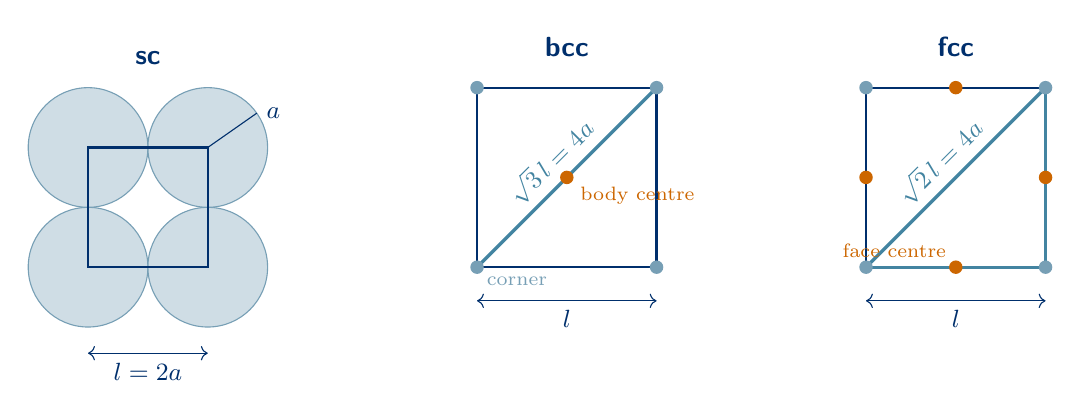
\begin{tikzpicture}[scale=0.95]
    % --- sc
    \begin{scope}
      \foreach \x/\y in {0/0, 1.6/0, 0/1.6, 1.6/1.6} {
        \fill[fautech!35] (\x,\y) circle (0.8);
        \draw[fautech] (\x,\y) circle (0.8);
      }
      \draw[faublue, thick] (0,0) rectangle (1.6,1.6);
      \draw[<->, faublue] (0,-1.15) -- (1.6,-1.15) node[midway, below] {\small $l = 2a$};
      \draw[faublue] (1.6,1.6) -- ++(35:0.8) node[right] {\small $a$};
      \node[faublue] at (0.8,2.8) {\sffamily\bfseries sc};
    \end{scope}
    % --- bcc
    \begin{scope}[xshift=5.2cm]
      \draw[faublue, thick] (0,0) rectangle (2.4,2.4);
      \draw[cyan!60!black, very thick] (0,0) -- (2.4,2.4);
      \foreach \x/\y in {0/0, 2.4/0, 0/2.4, 2.4/2.4} \fill[fautech] (\x,\y) circle (0.09);
      \fill[orange!80!black] (1.2,1.2) circle (0.09);
      \node[cyan!60!black, rotate=45, above, font=\small] at (1.2,1.2) {$\sqrt{3}\,l = 4a$};
      \draw[<->, faublue] (0,-0.45) -- (2.4,-0.45) node[midway, below] {\small $l$};
      \node[faublue] at (1.2,2.95) {\sffamily\bfseries bcc};
      \node[font=\scriptsize, fautech, below right] at (0,0) {corner};
      \node[font=\scriptsize, orange!80!black, below right] at (1.25,1.2) {body centre};
    \end{scope}
    % --- fcc
    \begin{scope}[xshift=10.4cm]
      \draw[faublue, thick] (0,0) rectangle (2.4,2.4);
      \draw[cyan!60!black, very thick] (0,0) -- (2.4,0) -- (2.4,2.4);
      \draw[cyan!60!black, very thick] (0,0) -- (2.4,2.4);
      \foreach \x/\y in {0/0, 2.4/0, 0/2.4, 2.4/2.4} \fill[fautech] (\x,\y) circle (0.09);
      \foreach \x/\y in {1.2/0, 0/1.2, 2.4/1.2, 1.2/2.4} \fill[orange!80!black] (\x,\y) circle (0.09);
      \node[cyan!60!black, rotate=45, above, font=\small] at (1.2,1.2) {$\sqrt{2}\,l = 4a$};
      \draw[<->, faublue] (0,-0.45) -- (2.4,-0.45) node[midway, below] {\small $l$};
      \node[faublue] at (1.2,2.95) {\sffamily\bfseries fcc};
      \node[font=\scriptsize, orange!80!black, above left] at (1.2,0) {face centre};
    \end{scope}
  \end{tikzpicture}
  \caption{The three cubic lattices and their close-packed directions. In sc the cube edge carries two
    radii from each of the two corner atoms; in bcc the body diagonal carries one corner atom, the body
    centre and the opposite corner, that is four radii; in fcc the face diagonal carries the two
    corners and the face centre, again four radii.}
  \label{fig:lattices}
\end{figure}

With $a = \SI{128}{\pico\metre}$ for copper this gives
\begin{equation}\label{eq:hardsphere}
  l_{\mathrm{sc}} = 2a = \SI{2.560}{\angstrom},
  \qquad
  l_{\mathrm{bcc}} = \frac{4a}{\sqrt3} = \SI{2.956}{\angstrom},
  \qquad
  l_{\mathrm{fcc}} = \frac{4a}{\sqrt2} = 2\sqrt2\,a = \SI{3.620}{\angstrom}.
\end{equation}
The fcc estimate is within $0.15\,\%$ of the experimental $\SI{3.615}{\angstrom}$, which is no accident
--- the metallic radius is \emph{defined} as half the nearest-neighbour distance in the close-packed
structure. The value of the estimate is as a starting point for the energy scan, not as a prediction.

\subsection{Molecular statics: structure and lattice constant (Task 3.2)}\label{sec:statics}

\begin{task}{3.2}
  Compute the minimal energies $W$ at 0\,K for the three cubic structures by molecular statics,
  starting from the estimates of Task~3.1. Fit the energy--lattice-constant data to a second-order
  polynomial $W = p_0 + p_1 l + p_2 l^2$, solve for the minimum $(l_0, W_0)$, and compare the lattice
  constant of the lowest-energy structure with the literature.
\end{task}

For each structure the lattice constant is scanned, the EMT energy per atom evaluated, and the
parabola $W = p_0 + p_1 l + p_2 l^2$ fitted, whose minimum lies at
\begin{equation}\label{eq:parabola}
  l_0 = -\frac{p_1}{2p_2},
  \qquad
  W_0 = p_0 - \frac{p_1^2}{4p_2}.
\end{equation}
\Cref{tab:lattice} collects the results of Part~II. EMT places fcc lowest, bcc
$\SI{0.037}{\electronvolt\per atom}$ above it and simple cubic a further
$\SI{0.42}{\electronvolt\per atom}$ higher --- the correct ordering, and the correct ground-state
structure for copper. Physically this reflects the many-body term of \cref{eq:emt}: the close-packed
structure has the highest coordination number (12, against 8 for bcc and 6 for sc) and therefore the
highest local electron density, which the concave embedding function rewards.

\begin{table}[ht]
  \centering
  \caption{Lattice constants and minimal energies from the EMT molecular statics of Part~II.
    $l_{\mathrm{est}}$ is the hard-sphere estimate of \cref{eq:hardsphere}, $l_{\mathrm{fit}}$ the
    minimum of the parabola fitted over the whole scan range, and $l_0$ the true minimum of the EMT
    energy. The energy zero of EMT is the equilibrium fcc crystal.}
  \label{tab:lattice}
  \begin{tabular}{lrrrrr}
    \toprule
    Structure & $l_{\mathrm{est}}$ [\AA] & $l_{\mathrm{fit}}$ [\AA] & $W_{\mathrm{fit}}$ [eV/atom]
      & $l_0$ [\AA] & $W_0$ [eV/atom] \\
    \midrule
    sc  & 2.560 & 2.426 & 0.4902 & 2.423 & 0.4520 \\
    bcc & 2.956 & 2.888 & 0.0776 & 2.842 & 0.0370 \\
    fcc & 3.620 & 3.650 & 0.0074 & \textbf{3.593} & \textbf{$-0.0016$} \\
    \bottomrule
  \end{tabular}
\end{table}

\paragraph{Comparison with the literature and a caveat about the fit.}
The experimental lattice constant of copper extrapolated to 0\,K is
$\SI{3.615}{\angstrom}$~\citep{straumanis1969} and the bulk modulus is about
$\SI{137}{\giga\pascal}$. EMT gives $l_0 = \SI{3.593}{\angstrom}$ ($-0.61\,\%$) and, from a
Birch--Murnaghan fit of the energy--volume curve, $B = \SI{134.3}{\giga\pascal}$ ($-2.0\,\%$). Both
quantities entered the parameterization, so this level of agreement is a consistency check rather than
a prediction.

The second-order fit requested by the task has a systematic bias that is worth stating. The EMT energy
curve is not a parabola: it is asymmetric, rising steeply under compression (the repulsive core) and
flattening under tension (the tail of the cohesive well). Fitted over the whole scan range the
parabola is pulled towards larger $l$, giving $\SI{3.650}{\angstrom}$ instead of
$\SI{3.593}{\angstrom}$ --- an error of $1.6\,\%$, three times the error of the potential itself.
Restricting the fit to $\pm\SI{0.25}{\angstrom}$ around the minimum, or using a Birch--Murnaghan
equation of state, removes the bias. The same anharmonicity is the subject of Task~3.6
(\cref{sec:quadratic}), and it is the reason the elastic constants below are extracted from a narrow
strain window with a third-order rather than a second-order fit.

% ===============================================================
\section{Elastic constants}\label{sec:elastic}
% ===============================================================

The elastic constants are the second derivatives of the strain energy density with respect to the
strain,
\begin{equation}\label{eq:stiffness}
  \bsig = \frac{\partial \We}{\partial\beps},
  \qquad
  \We = \frac{1}{2}\,\beps : \CC : \beps,
  \qquad
  \CC = \frac{\partial^2 \We}{\partial\beps^2},
\end{equation}
so that each independent component can be read off from the energy of a suitably chosen homogeneous
deformation. In Voigt notation the energy of a general strain state is
\begin{equation}\label{eq:voigtenergy}
  \We = \frac{1}{2}\,\varepsilon^{\mathrm{v}}_\alpha\,C^{\mathrm{v}}_{\alpha\beta}\,
        \varepsilon^{\mathrm{v}}_\beta,
\end{equation}
with the convention $\varepsilon^{\mathrm{v}} = (\varepsilon_{11},\varepsilon_{22},\varepsilon_{33},
2\varepsilon_{23},2\varepsilon_{13},2\varepsilon_{12})^{\mathsf T}$. Evaluating \cref{eq:voigtenergy}
for a chosen $\varepsilon^{\mathrm{v}}$ gives one equation per deformation.

\subsection{Strain states for an isotropic material (Task 3.3)}\label{sec:isotropic}

\begin{task}{3.3}
  Write down the equations for the missing elastic constants and give a possible strain distribution
  for each, using already computed constants where helpful. Assume first an isotropic material, for
  which $C_{44} = (C_{11}-C_{12})/2$.
\end{task}

An isotropic solid has only two independent constants. Inserting the uniaxial state
$\varepsilon^{\mathrm{v}} = (\epsb,0,0,0,0,0)^{\mathsf T}$ into \cref{eq:voigtenergy} leaves a single
term, which is the relation given in the script:
\begin{equation}\label{eq:C11}
  \We = \frac{1}{2}\,C_{11}\,\epsb^2
  \qquad\Longrightarrow\qquad
  \boxed{\;C_{11} = \frac{2\We}{\epsb^2}.\;}
\end{equation}
For $C_{12}$ a state is needed in which two normal strains act at once, so that the off-diagonal block
of the stiffness matrix is activated. The \emph{biaxial} state
$\varepsilon^{\mathrm{v}} = (\epsb,\epsb,0,0,0,0)^{\mathsf T}$ gives
\begin{equation}\label{eq:biax}
  \We = \frac{1}{2}\left(C_{11}\epsb^2 + C_{12}\epsb^2 + C_{12}\epsb^2 + C_{11}\epsb^2\right)
      = \left(C_{11}+C_{12}\right)\epsb^2
  \qquad\Longrightarrow\qquad
  \boxed{\;C_{12} = \frac{\We}{\epsb^2} - C_{11}.\;}
\end{equation}
The hydrostatic state $\varepsilon^{\mathrm{v}} = (\epsb,\epsb,\epsb,0,0,0)^{\mathsf T}$ provides an
independent route and at the same time the bulk modulus,
\begin{equation}\label{eq:hydro}
  \We = \frac{3}{2}\left(C_{11}+2C_{12}\right)\epsb^2 = \frac{9}{2}B\,\epsb^2,
  \qquad
  B = \frac{C_{11}+2C_{12}}{3},
\end{equation}
which we use in Part~II as a consistency check on the two preceding results. For an isotropic material
the shear constant follows without further computation,
\begin{equation}\label{eq:C44iso}
  C_{44} = \frac{C_{11}-C_{12}}{2} = \mu,
\end{equation}
which is the Lam\'e shear modulus; $C_{12} = \lambda$ completes the pair.

\subsection{Strain states for cubic symmetry (Task 3.4)}\label{sec:cubic}

\begin{task}{3.4}
  In the same manner write down the equations and the strain distribution for a material with cubic
  symmetry, for which $C_{11}$, $C_{12}$ and $C_{44}$ are independent.
\end{task}

In a cubic crystal \cref{eq:C44iso} no longer holds and $C_{44}$ must be measured. A pure shear in the
$2$--$3$ plane, $\varepsilon^{\mathrm{v}} = (0,0,0,\epsb,0,0)^{\mathsf T}$, that is
$\varepsilon_{23} = \varepsilon_{32} = \epsb/2$ in tensor components, activates only the $C_{44}$
entry:
\begin{equation}\label{eq:C44}
  \We = \frac{1}{2}\,C_{44}\,\epsb^2
  \qquad\Longrightarrow\qquad
  \boxed{\;C_{44} = \frac{2\We}{\epsb^2},\;}
  \qquad
  \beps = \begin{pmatrix} 0 & 0 & 0 \\ 0 & 0 & \epsb/2 \\ 0 & \epsb/2 & 0\end{pmatrix}.
\end{equation}
\Cref{eq:C11,eq:biax,eq:C44} are a complete set for cubic symmetry, with \cref{eq:hydro} as a check.
The degree of anisotropy is measured by the Zener ratio
\begin{equation}\label{eq:zener}
  A = \frac{2C_{44}}{C_{11}-C_{12}},
\end{equation}
which equals one exactly for an isotropic material by \cref{eq:C44iso}; copper has $A \approx 3.2$ and
is one of the most elastically anisotropic cubic metals.

\paragraph{Implementation.}
In ASE the cell is a $3\times3$ matrix of row vectors, and a homogeneous deformation is applied by
multiplying it with $\bI + \beps$ while scaling the atomic positions by the same map. For the uniaxial
state,
\begin{equation}\label{eq:celldef}
  \underbrace{\begin{pmatrix} l_0 & 0 & 0\\ 0 & l_0 & 0\\ 0&0&l_0\end{pmatrix}}_{\text{optimal cell}}
  \left(
  \underbrace{\begin{pmatrix} \epsb & 0 & 0\\ 0&0&0\\ 0&0&0\end{pmatrix}}_{\beps}
  + \bI \right)
  = \underbrace{\begin{pmatrix} l_0(1+\epsb) & 0 & 0\\ 0 & l_0 & 0\\ 0&0&l_0\end{pmatrix}}
    _{\text{deformed cell}} .
\end{equation}
Rather than evaluating \cref{eq:C11,eq:biax,eq:C44} at a single strain, we follow the script and record
a whole energy--strain curve, fit it with a third-order polynomial
$\We = p_0 + p_1\epsb + p_2\epsb^2 + p_3\epsb^3$, and evaluate the curvature at the minimum,
\begin{equation}\label{eq:d2W}
  \frac{\mathrm{d}^2\We}{\mathrm{d}\epsb^2} = 2p_2 + 6p_3\,\epsb_{\min}.
\end{equation}
The cubic term absorbs the leading anharmonicity and the position of the minimum serves as a diagnostic:
if the reference cell is properly relaxed, $\epsb_{\min}$ must come out at zero. In Part~II it does, to
within $10^{-6}$, which confirms that the deformations start from the true energy minimum.

\subsection{Results for fcc copper (Task 3.5)}\label{sec:results-elastic}

\begin{task}{3.5}
  Evaluate the elastic constants of copper in the fcc configuration using the deformation states above,
  starting from the relaxed cell at $l_0$. Compare the results with the 0\,K literature values and give
  the error in percent for each constant.
\end{task}

\begin{table}[ht]
  \centering
  \caption{Elastic constants of fcc copper from EMT (Part~II) compared with the 0\,K single-crystal
    measurements of Overton and Gaffney~\citep{overton1955}.}
  \label{tab:elastic}
  \begin{tabular}{lrrr}
    \toprule
     & EMT [GPa] & Experiment, 0\,K [GPa] & Error \\
    \midrule
    $C_{11}$ & 173.0 & 176.2 & $-1.8\,\%$ \\
    $C_{12}$ & 116.3 & 124.9 & $-6.9\,\%$ \\
    $C_{44}$ &  89.9 &  81.8 & $+9.9\,\%$ \\
    \midrule
    $B = (C_{11}+2C_{12})/3$ & 135.2 & 142.0 & $-4.8\,\%$ \\
    $A = 2C_{44}/(C_{11}-C_{12})$ & 3.17 & 3.19 & $-0.6\,\%$ \\
    $C_{12}/C_{44}$ (Cauchy: 1) & 1.29 & 1.53 & --- \\
    \bottomrule
  \end{tabular}
\end{table}

\Cref{tab:elastic} gives the result. Three observations.

First, the errors are not random but ordered: $C_{11}$ and the bulk modulus, which are directly tied to
the quantities EMT was fitted to, come out within a few percent, whereas $C_{12}$ and especially
$C_{44}$ --- shear responses that were not part of the fit --- are off by $7$ and $10\,\%$. This is the
practical consequence of \cref{sec:fitting}: a potential is accurate where it was fitted and only
plausible elsewhere.

Second, the qualitative physics is right. The Cauchy relation \cref{eq:cauchy} is strongly violated
($C_{12}/C_{44} = 1.29$ instead of $1$), which no pair potential could achieve, and the Zener
anisotropy is reproduced almost exactly. If the question is whether copper is elastically anisotropic
and by how much, EMT answers it correctly; if the question is the absolute value of the shear modulus
to better than $10\,\%$, a fitted EAM potential is required.

Third, the two errors partially cancel in the bulk modulus, because $B$ depends on $C_{11}+2C_{12}$,
which was fitted, while the error lives in the deviatoric combination $C_{11}-C_{12}$.

% ===============================================================
\section{Validity of the quadratic assumption (Task 3.6)}\label{sec:quadratic}
% ===============================================================

\begin{task}{3.6}
  We assumed a quadratic dependence of the energy density on the strains. By looking at the strain
  energy plots, estimate the range around the relaxed state for which this assumption is reasonable.
\end{task}

The whole construction of \cref{sec:elastic} rests on $\We = \tfrac12 C\epsb^2$, which is the second
order term of a Taylor expansion about the relaxed state. Part~II measures the departure from it by
comparing the computed energy with the parabola built from the constants of \cref{tab:elastic}:
\begin{equation}\label{eq:validity}
  \frac{\left|\We(\epsb) - \tfrac12 C\epsb^2\right|}{\tfrac12 C\epsb^2} < 5\,\%
  \qquad\Longrightarrow\qquad
  \begin{cases}
    |\epsb| \lesssim 3.5\,\% & \text{uniaxial},\\[2pt]
    |\epsb| \lesssim 14.5\,\% & \text{shear}.
  \end{cases}
\end{equation}
Two features deserve comment.

\paragraph{The uniaxial curve is asymmetric.}
Compression drives the atoms into the steeply rising repulsive core of the potential, tension into the
flat tail of the cohesive well, so the energy grows much faster on the compressive side. The leading
correction to the quadratic law is therefore the \emph{cubic} term, which is exactly the $p_3$ that the
third-order fit of \cref{eq:d2W} was introduced to absorb. The practical consequence is that a
one-sided or badly centred strain window biases the extracted constant, which is also what happened to
the second-order fit of the lattice constant in \cref{sec:statics}.

\paragraph{Shear stays quadratic much longer.}
For a shear of a cubic crystal $\We(\epsb) = \We(-\epsb)$ by symmetry --- shearing the $2$--$3$ plane in
one direction is crystallographically equivalent to shearing it in the other --- so all odd terms of
the expansion vanish identically and the first correction is quartic. This is visible both in the plot
of Part~II and in the fitted $\epsb_{\min} \approx 10^{-14}$ for the shear state.

\paragraph{Choice of the strain window.}
A window of $\pm2\,\%$, used throughout Part~II, is therefore a compromise: wide enough that the energy
differences are large against the numerical noise of the calculator ($\sim10^{-8}$ eV), narrow enough
that the cubic correction is a small perturbation. A real material fails long before leaving this
window --- copper yields at an elastic strain of a few tenths of a percent --- so linear elasticity is
not merely a numerical convenience but an excellent description of the accessible range. The nanotube
of the next section is the exception that proves the rule: it sustains elastic strains of tens of
percent and is strongly nonlinear long before it breaks.

% ===============================================================
\section{Molecular dynamics of a carbon nanotube}\label{sec:cnt}
% ===============================================================

\subsection{Nanotube types and chirality (Task 4.1)}\label{sec:cnttypes}

\begin{task}{4.1}
  Look up what kinds of carbon nanotube exist, how they are specified and what their structure looks
  like. Can you estimate the mechanical behaviour from the structure alone, with respect to anisotropy
  and the pattern of the carbon atoms? For the following tasks choose a $(5,5)$ armchair nanotube.
\end{task}

A single-walled carbon nanotube is a graphene sheet rolled into a cylinder. The roll-up is specified
by the chiral vector
\begin{equation}\label{eq:chiral}
  \bm{C}_h = n\,\bm{a}_1 + m\,\bm{a}_2,
\end{equation}
with the graphene lattice vectors $\bm{a}_1, \bm{a}_2$ and the integers $(n,m)$. The circumference is
$|\bm{C}_h|$, so the diameter and the chiral angle are
\begin{equation}\label{eq:diameter}
  d = \frac{a_{\mathrm{cc}}\sqrt{3\left(n^2+nm+m^2\right)}}{\pi},
  \qquad
  \theta = \arctan\frac{\sqrt3\,m}{2n+m},
  \qquad a_{\mathrm{cc}} = \SI{1.42}{\angstrom}.
\end{equation}
Three families follow from the value of $\theta$: \emph{armchair} tubes with $m = n$
($\theta = 30^\circ$), \emph{zigzag} tubes with $m = 0$ ($\theta = 0^\circ$), and \emph{chiral} tubes
otherwise. The electronic structure follows a simple rule: the tube is metallic if $n-m$ is divisible
by three and semiconducting otherwise, so all armchair tubes are metals. The $(5,5)$ tube used here has
$d = \SI{6.78}{\angstrom}$, $\theta = 30^\circ$ and is metallic.

\paragraph{Mechanical behaviour from the structure.}
The bonds are not isotropically distributed, and the pattern tells us what to expect.
\begin{itemize}\setlength{\itemsep}{2pt}
  \item In an \emph{armchair} tube one third of the C--C bonds lie exactly perpendicular to the tube
    axis and carry no axial load; the other two thirds are inclined at $\pm30^\circ$. Axial tension
    therefore loads these bonds in a mixed stretching/bond-angle mode, and part of the strain is
    accommodated by \emph{straightening} the zigzag path rather than by stretching bonds.
  \item In a \emph{zigzag} tube the situation is reversed: one third of the bonds lie along the axis
    and take the load in pure stretching.
\end{itemize}
Bond stretching is much stiffer than bond bending, so a zigzag tube is axially stiffer and fails at a
smaller strain, whereas an armchair tube reaches a larger failure strain. The tube is therefore
mechanically anisotropic --- stiff along the axis, soft in bending and radial compression --- and the
chirality controls both the stiffness and the failure strain. The sp$^2$ bond itself is one of the
strongest in nature, which is why the predicted Young's modulus is of the order of $\SI{1}{\tera\pascal}$,
five times that of steel at one fifth of the density.

\subsection{Time step, relaxation time and the critical deformation rate (Task 4.2)}\label{sec:rate}

\begin{task}{4.2}
  Estimate a critical deformation rate at which the system has not enough time to relax and becomes
  unstable. Stretch the tube along its axis in an NVE ensemble with the velocity-Verlet integrator,
  starting from the relaxed state at 0\,K and deforming incrementally. Start with a small time step
  (e.g.\ $\SI{0.1}{\femto\second}$) and investigate the relaxation time. How does it change for larger
  steps? For a given deformation rate, is it better to take many small steps with short relaxations or
  a few large steps with long relaxations?
\end{task}

\paragraph{The time step.}
Velocity-Verlet is a symplectic integrator: it conserves a shadow Hamiltonian and therefore shows no
secular energy drift, \emph{provided} the time step resolves the fastest oscillation present. For
carbon that is the C--C stretching mode. Part~II measures the drift of an unforced NVE run at fixed
strain and finds it below $\SI{0.01}{\milli\electronvolt\per atom}$ over $\SI{400}{\femto\second}$ for
$\Delta t \le \SI{1}{\femto\second}$, rising by more than an order of magnitude at
$\Delta t = \SI{4}{\femto\second}$. All production runs use $\Delta t = \SI{0.5}{\femto\second}$.

\paragraph{The relaxation time.}
After a $1\,\%$ step strain the potential energy of the tube oscillates with a dominant frequency of
$\SI{100}{\tera\hertz}$, i.e. a period of $\tau = \SI{10}{\femto\second}$. Since the energy is
quadratic in the displacement, the underlying displacement mode is at half that frequency,
$\SI{50}{\tera\hertz}$, which is the C--C stretching mode --- the graphite $G$ band lies at
$1580\,\mathrm{cm^{-1}} \approx \SI{47}{\tera\hertz}$, so the Brenner potential reproduces it well. The
usual stability criterion $\Delta t < T_{\mathrm{osc}}/20 = \SI{1}{\femto\second}$ is consistent with
the measured drift.

It is worth being precise about what ``relaxation'' means here. The tube in NVE is an isolated,
nearly harmonic system: a step strain does not decay, it excites a coherent oscillation that only
dephases as the anharmonic couplings spread the energy over the other modes. The relevant time scale
is nevertheless $\tau$, because only after several periods has the injected elastic energy been
redistributed and can the structure be said to have followed the deformation. Larger strain steps do
not change $\tau$, which is a material property, but they increase the amplitude --- the injected energy
scales as $\Delta\varepsilon^2$ --- and thereby push the system into the anharmonic regime where the
dephasing is faster but uncontrolled.

\paragraph{The critical deformation rate.}
Quasi-static behaviour requires the time spent per strain increment to be long compared with $\tau$,
which gives
\begin{equation}\label{eq:ratecrit}
  \dot\varepsilon_{\mathrm{crit}} \sim \frac{\varepsilon_{\mathrm{el}}}{\tau}
  \approx \frac{0.1}{\SI{10}{\femto\second}} = 10^{13}\,\mathrm{s^{-1}}
\end{equation}
as an upper bound, reduced by one to two orders of magnitude because the energy must be redistributed
over several periods. \Cref{tab:rates} gives the measurement of Part~II: up to
$2\cdot10^{11}\,\mathrm{s^{-1}}$ the dynamic energy--strain curves lie on the quasi-static path to
within $\SI{0.04}{\milli\electronvolt\per atom}$ and the failure strain is rate independent, whereas
above $\sim10^{12}\,\mathrm{s^{-1}}$ the deviation grows by two orders of magnitude and the apparent
failure strain rises from $0.41$ to $0.50$. The critical rate is therefore
$\dot\varepsilon_{\mathrm{crit}} \approx 10^{12}\,\mathrm{s^{-1}}$, consistent with
\cref{eq:ratecrit}. Above it the tube is pulled through the instability before the atoms can rearrange
into the broken-bond configuration, so failure is artificially \emph{delayed} and the stored energy at
failure is too high.

\begin{table}[ht]
  \centering
  \caption{Rate dependence of the tensile failure of the $(5,5)$ tube in NVE at 0\,K (Part~II). The
    last column is the maximum deviation of the dynamic energy from the quasi-static path for
    $\varepsilon < 0.3$.}
  \label{tab:rates}
  \begin{tabular}{rrrr}
    \toprule
    $\dot\varepsilon$ [s$^{-1}$] & MD steps & $\varepsilon$ at failure & deviation [meV/atom] \\
    \midrule
    $4\cdot10^{10}$ & \num{24999} & 0.407 & 0.02 \\
    $1\cdot10^{11}$ & \num{10000} & 0.420 & 0.04 \\
    $2\cdot10^{11}$ & \num{5000}  & 0.430 & 0.02 \\
    $6\cdot10^{11}$ & \num{1666}  & 0.437 & 0.79 \\
    $2\cdot10^{12}$ & \num{500}   & 0.472 & 5.24 \\
    $6\cdot10^{12}$ & \num{166}   & 0.498 & 8.08 \\
    \midrule
    quasi-static (relaxed) & --- & 0.33 & --- \\
    \bottomrule
  \end{tabular}
\end{table}

\begin{remark}
  Even the slowest rate in \cref{tab:rates} is fifteen orders of magnitude faster than a laboratory
  tensile test at $10^{-3}\,\mathrm{s^{-1}}$. This rate gap is the fundamental limitation of molecular
  dynamics: the time step is set by the atomic vibration period, so reaching a second of physical time
  would take $10^{15}$ steps. It is the reason accelerated sampling methods exist, and the direct
  motivation for the kinetic Monte Carlo method of Practical~6, which replaces the vibrations by
  transition rates and thereby reaches laboratory time scales.
\end{remark}

\paragraph{Many small steps or a few large ones?}
For a given average deformation rate, many small increments with short relaxations are clearly
preferable. The elastic energy injected by one increment scales as $\Delta\varepsilon^2$, so a step ten
times larger injects a hundred times the energy at once; that energy appears as a coherent,
large-amplitude oscillation that drives the bonds into the anharmonic region and can trigger a failure
that has nothing to do with the applied strain level. Small increments keep the perturbation inside
the harmonic regime, where the system follows the deformation adiabatically --- and they cost nothing
extra, because the total number of MD steps at a given rate is the same either way.

\subsection{Energy increase under deformation (Task 4.3)}\label{sec:energy}

\begin{task}{4.3}
  Calculate the energy increase induced by the deformation and plot the energy over the deformation.
  What happens to the kinetic, potential and total energy at large deformations?
\end{task}

Three regimes are visible in the plots of Part~II.

\begin{enumerate}\setlength{\itemsep}{3pt}
  \item \textbf{Elastic and anharmonic loading.} Essentially all the external work goes into potential
    energy. The kinetic energy stays near zero and the tube remains at a few kelvin: an affine
    rescaling of a relaxed structure is close to the minimum energy path, so almost no vibration is
    excited. The potential energy rises to
    $\Delta E = \SI{2.54}{\electronvolt\per atom}$ at the instability.
  \item \textbf{Failure.} The first bonds break. The potential energy drops sharply and, because the
    simulation is NVE, the released energy has nowhere to go but into kinetic energy: $E_{\mathrm{kin}}$
    jumps from $\SI{2.5}{\electronvolt}$ to $\SI{169}{\electronvolt}$ and the temperature spikes from
    $\SI{97}{\kelvin}$ to over $\SI{6500}{\kelvin}$. The fracture site effectively melts.
  \item \textbf{The total energy increases monotonically.} This is \emph{not} an integrator drift ---
    \cref{sec:rate} established that the drift is below
    $\SI{0.01}{\milli\electronvolt\per atom}$. It is the external work done by the moving cell
    boundary, which is the one channel through which energy enters an otherwise microcanonical run with
    a time-dependent cell. Over the whole run the cell does $\SI{551}{\electronvolt}$ of work on the
    tube.
\end{enumerate}

\subsection{NVT tension test at 300\,K (Task 4.4)}\label{sec:nvt}

\begin{task}{4.4}
  Use an NVT ensemble to perform the uniaxial deformation test at constant $T = \SI{300}{\kelvin}$.
  Compare the energies of the two systems. What can be observed?
\end{task}

Coupling the tube to a Langevin heat bath changes the picture in three ways.

\begin{enumerate}\setlength{\itemsep}{3pt}
  \item \textbf{The thermostatted tube fails earlier}, at $\varepsilon = 0.408$ against $0.430$ in NVE
    at 0\,K. At 300\,K the atoms already carry thermal displacements of a few hundredths of an
    \AA ngstr\"om, so at any instant some bond somewhere along the tube is closer to its breaking
    configuration than it would be at 0\,K. Failure is a thermally activated event and the fluctuation
    supplies part of the barrier. This is the atomistic version of the familiar statement that strength
    decreases with temperature.
  \item \textbf{Less energy is stored at failure}, $\SI{2.26}{\electronvolt\per atom}$ against
    $\SI{2.54}{\electronvolt\per atom}$, for the same reason; and the energy--strain curve is offset by
    the thermal energy $\tfrac32\kB T \approx \SI{39}{\milli\electronvolt\per atom}$ and is visibly
    noisier.
  \item \textbf{The total energy behaves completely differently.} In NVE it can only grow, because the
    deformation work has nowhere to go; in NVT the thermostat removes that work continuously, the total
    energy stays flat during loading and does not spike at fracture. Physically, the NVT run describes
    an isothermal specimen in contact with its surroundings --- a room-temperature tensile test ---
    whereas the NVE run describes a perfectly insulated, adiabatic one in which the fracture heat
    cannot escape and melts the specimen.
\end{enumerate}

\subsection{Bond-breaking energy and the stress--strain curve (Task 4.5)}\label{sec:bond}

\begin{task}{4.5}
  Calculate the bond-breaking energy of a carbon nanotube with the Brenner potential at room
  temperature. How can a stress--strain curve be obtained from the calculations?
\end{task}

\paragraph{From energy to stress.}
A molecular dynamics run delivers energies, not stresses. For a homogeneous deformation the two are
connected by the derivative of the stored energy,
\begin{equation}\label{eq:stressfromE}
  \sigma(\varepsilon) = \frac{1}{V_0}\,\frac{\mathrm{d}U}{\mathrm{d}\varepsilon},
\end{equation}
so the stress--strain curve follows from numerically differentiating the quasi-static energy--strain
curve, and Young's modulus is the curvature at the origin,
$E = V_0^{-1}\,\mathrm{d}^2U/\mathrm{d}\varepsilon^2|_{\varepsilon=0}$. (The virial stress of the
calculator is an independent route to the same quantity.)

The only ambiguity is $V_0$. A nanotube is a surface, not a solid, and there is no unique way to assign
it a volume; the convention is to give the wall the graphite interlayer spacing
$t = \SI{3.4}{\angstrom}$, so that
\begin{equation}\label{eq:volume}
  V_0 = 2\pi R\,t\,L_0.
\end{equation}
Every reported modulus and strength of a nanotube depends on this choice, which is why the literature
also quotes the thickness-independent \emph{surface} modulus $Et$ in $\si{\giga\pascal\nano\metre}$.
The numerical values are given in Part~II.

\paragraph{Bond-breaking energy.}
Part~II reports three complementary measures, because ``the'' bond-breaking energy is not a single
number.
\begin{enumerate}\setlength{\itemsep}{2pt}
  \item \emph{From cohesion.} The relaxed tube has $\SI{-7.245}{\electronvolt\per atom}$ and
    $3/2$ bonds per atom, so one C--C bond is worth about $\SI{4.8}{\electronvolt}$ --- in good
    agreement with the sp$^2$ bond energy of graphene ($\approx\SI{4.9}{\electronvolt}$), which is what
    the Brenner potential was fitted to reproduce.
  \item \emph{From fracture.} Relaxing the broken tube and comparing it with the intact one gives the
    energy actually spent on creating the two new ends, and dividing by the number of bonds that were
    lost gives the energy per broken bond. It is smaller than the cohesive estimate, because the atoms
    at the new edge rebond and partially recover their energy --- the same many-body effect that makes
    the vacancy formation energy smaller than the cohesive energy in \cref{sec:pairfail}.
  \item \emph{As a fracture energy.} Dividing the same quantity by twice the cross-sectional area
    $2\pi Rt$ gives a surface energy $\gamma$ that can be compared with the cleavage energy of graphite.
\end{enumerate}

\paragraph{A caveat on the first-generation Brenner potential.}
The failure strains reported in \cref{tab:rates} ($0.33$ quasi-statically, $0.41$--$0.50$ dynamically)
and the corresponding peak stresses are substantially higher than the values from DFT or from the
later REBO/AIREBO parameterizations. The reason is known and specific: the original Brenner
potential~\citep{brenner1990} switches the bond off with a cut-off function between $\SI{1.7}{\angstrom}$
and $\SI{2.0}{\angstrom}$. A stretched bond passing through this window experiences an artificial
restoring force from the derivative of the switching function, which stiffens the bond just before it
should break and pushes both the fracture strain and the peak stress up~\citep{shenderova2000}. The
numbers in this section are therefore quantitatively unreliable as predictions of real nanotube
strength, although the trends --- the rate dependence, the temperature dependence, the shape of the
energy--strain curve --- are robust. This is a concrete instance of the general warning of
\cref{sec:fitting}: the potential is being used outside the configuration space it was fitted in.

% ===============================================================
\section{Conclusion}\label{sec:conclusion}
% ===============================================================

The three families of empirical potential differ in one essential respect: whether the energy of a bond
depends on the environment of the atoms that form it. A pair potential says no, and as a consequence
obeys the Cauchy relation $C_{12} = C_{44}$ exactly, predicts a vacancy formation energy equal to the
cohesive energy and relaxes metal surfaces the wrong way --- three qualitative failures that no choice
of parameters can repair. EAM and EMT both say yes, by embedding each atom in the electron density of
its neighbours; EMT derives that construction from the effective-medium theory with seven physically
meaningful parameters, EAM postulates it with tabulated functions fitted to a large experimental
database. The trade-off is flexibility against transferability.

Verifying EMT for copper confirms both its strengths and the limits of that trade-off. The correct
ground-state structure is found (fcc, below bcc and simple cubic), the lattice constant comes out at
$\SI{3.593}{\angstrom}$ against the measured $\SI{3.615}{\angstrom}$ and the bulk modulus at
$\SI{134}{\giga\pascal}$ against $\SI{137}{\giga\pascal}$. The elastic constants
$C_{11} = \SI{173.0}{\giga\pascal}$, $C_{12} = \SI{116.3}{\giga\pascal}$ and
$C_{44} = \SI{89.9}{\giga\pascal}$ deviate by $-1.8$, $-6.9$ and $+9.9$ percent --- small errors where
the potential was fitted, larger ones where it was not --- while the Cauchy violation and the Zener
anisotropy, the qualitative signatures of metallic bonding, are reproduced. The quadratic energy--strain
law on which all of this rests holds to within $5\,\%$ for uniaxial strains below about $3.5\,\%$, and
much further in shear, where symmetry removes the cubic term.

The molecular dynamics of the $(5,5)$ nanotube illustrates the two characteristic difficulties of the
method. The first is the time step: it must resolve the C--C stretching mode, whose period we measured
as $\SI{10}{\femto\second}$ in the energy, which limits $\Delta t$ to about $\SI{1}{\femto\second}$ and
makes laboratory time scales unreachable. The second is the deformation rate: below about
$10^{11}\,\mathrm{s^{-1}}$ the tube follows the quasi-static path, above about
$10^{12}\,\mathrm{s^{-1}}$ it does not and the failure strain becomes an artefact of the loading rate.
Within those limits the physics is sensible --- thermal fluctuations lower the failure strain from
$0.43$ at 0\,K to $0.41$ at 300\,K, and in NVE the bond-breaking energy is released as heat that raises
the local temperature above $\SI{6000}{\kelvin}$, whereas in NVT the thermostat carries it away. The
absolute failure strains and strengths, however, are inflated by the cut-off artefact of the
first-generation Brenner potential, which is a reminder that the most important step of an atomistic
simulation is the one taken before any atom is moved: choosing, and verifying, the potential.

% ===============================================================
\begin{thebibliography}{99}
% ===============================================================

\bibitem{script4}
Institute of Materials Simulation (WW8),
``Atomistic simulation,''
Materials Simulation Practical No.~4, tutorial script,
Friedrich-Alexander-Universit\"at Erlangen-N\"urnberg.

\bibitem{allen2017}
M.~P.~Allen and D.~J.~Tildesley,
\textit{Computer Simulation of Liquids},
2nd~ed.,
Oxford University Press, Oxford, 2017.

\bibitem{daw1984}
M.~S.~Daw and M.~I.~Baskes,
``Embedded-atom method: Derivation and application to impurities, surfaces, and other defects in
metals,''
\textit{Physical Review B},
vol.~29, no.~12, pp.~6443--6453, 1984.

\bibitem{jacobsen1987}
K.~W.~Jacobsen, J.~K.~N{\o}rskov and M.~J.~Puska,
``Interatomic interactions in the effective-medium theory,''
\textit{Physical Review B},
vol.~35, no.~14, pp.~7423--7442, 1987.

\bibitem{jacobsen1996}
K.~W.~Jacobsen, P.~Stoltze and J.~K.~N{\o}rskov,
``A semi-empirical effective medium theory for metals and alloys,''
\textit{Surface Science},
vol.~366, no.~2, pp.~394--402, 1996.

\bibitem{foiles1986}
S.~M.~Foiles, M.~I.~Baskes and M.~S.~Daw,
``Embedded-atom-method functions for the fcc metals Cu, Ag, Au, Ni, Pd, Pt, and their alloys,''
\textit{Physical Review B},
vol.~33, no.~12, pp.~7983--7991, 1986.

\bibitem{mishin2001}
Y.~Mishin, M.~J.~Mehl, D.~A.~Papaconstantopoulos, A.~F.~Voter and J.~D.~Kress,
``Structural stability and lattice defects in copper: Ab initio, tight-binding, and embedded-atom
calculations,''
\textit{Physical Review B},
vol.~63, no.~22, 224106, 2001.

\bibitem{brenner1990}
D.~W.~Brenner,
``Empirical potential for hydrocarbons for use in simulating the chemical vapor deposition of diamond
films,''
\textit{Physical Review B},
vol.~42, no.~15, pp.~9458--9471, 1990.

\bibitem{shenderova2000}
O.~A.~Shenderova, V.~V.~Zhirnov and D.~W.~Brenner,
``Carbon nanostructures,''
\textit{Critical Reviews in Solid State and Materials Sciences},
vol.~27, no.~3--4, pp.~227--356, 2002.

\bibitem{overton1955}
W.~C.~Overton and J.~Gaffney,
``Temperature variation of the elastic constants of cubic elements.~I.~Copper,''
\textit{Physical Review},
vol.~98, no.~4, pp.~969--977, 1955.

\bibitem{straumanis1969}
M.~E.~Straumanis and L.~S.~Yu,
``Lattice parameters, densities, expansion coefficients and perfection of structure of Cu and of
Cu--In $\alpha$ phase,''
\textit{Acta Crystallographica A},
vol.~25, no.~6, pp.~676--682, 1969.

\bibitem{ase2017}
A.~H.~Larsen et al.,
``The atomic simulation environment --- a Python library for working with atoms,''
\textit{Journal of Physics: Condensed Matter},
vol.~29, no.~27, 273002, 2017.

\bibitem{asap}
ASAP --- As Soon As Possible, a calculator for ASE,
Technical University of Denmark,
\url{https://wiki.fysik.dtu.dk/asap}.

\end{thebibliography}

\end{document}
